\section{Abstract model for DAE units}

In this section we will introduce a simplifying model for Winfree's solution to the $\mathsf{HPP}$. We have two reasons:
\begin{enumerate}   %!% opravdu to jsou ty důvody?? s rezervou ...
	\item the model will be based on the $\atam$ model,
	\item pictures will be easier-to-read.
\end{enumerate}

\begin{defn}
	Let us define $\myatam$ (augmented $\atam$) as $\atam$ where:
	\begin{itemize}
		\item temperature is set to $\tau = 2$,
		\item there are another $5$ tile shapes\footnote{Even with their vertical reflections.}, see Figure \ref{fig:abstract_model} (tiles {\sf ADEB}, {\sf CA}, {\sf KG}, {\sf KLO} and {\sf OP DONE}),
		\item glue strengths are restricted to corresponding tile type, all of which appear in Figure \ref{fig:abstract_model}.
	\end{itemize}
\end{defn}

\begin{note}
	Note that $\myatam$ can be easily simulated by classical $\atam$.
\end{note}

%%%%%%%%%%%%%%%%%%%%%%%%%%%%%%%%%%%%%%%%%%%%%%%%%%%%%%%%%%%%%%%%%%%%%%%%

\begin{remark}   %!% kam s tim?
	Those bottom tiles with glue-strength $2$ will be used for generating random words. Note that these words can be restricted by arbitrary regular grammar rule.
\end{remark}

%!% popsat co znamená že je něco sestavitelný -- NP, že má něco pst sestavení -- BPP

Note those twice longer sticky ends on the bottom line.

In following examples this model will be set up to act similarly like $\NP$: $\exists y \; R(x,y)$. Although existence is not sure, it is very likely. Predicate $R$ will be ``enumerable in polynomial time'' for $x \in L$. In this context, {\em enumerable in polynomial time} will mean number of bindings, not number of biosteps. This can be assumed due to Turing universality of this model in $O(1)$ biosteps -- biostep complexity is not restrictive\footnote{From Turing's thesis, Turing machine is the most universal model.} and will be required to be $O(1)$ due to its lab complexity. On the other hand the binding complexity will be very important, we will be interested even in constants. This is because the less binding complexity, the less probability of error.

Note that the word on the bottom line can be restricted to belong to arbitrary regular language.

%!% odhady se dají zmenšit pomocí #E místo #V^2
%!% spodní řádek má 2x tak dlouhý lepidla !! vysvětlit proč

\begin{figure}[H]
\begin{center}
	\begin{subfigure}[b]{0.31\textwidth}
		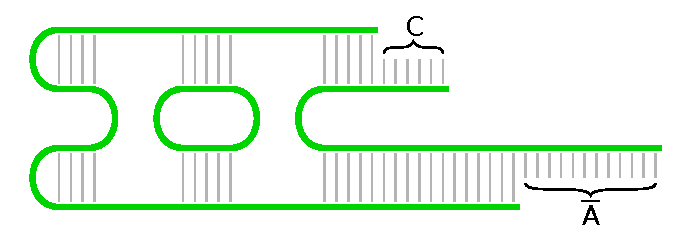
\includegraphics[width=\textwidth]{./figures/tile_model/DNA_struct.pdf} % 115mm
		\caption{Corner DAE unit}
		\label{fig:DNA_struct}
	\end{subfigure}
	\begin{subfigure}[b]{0.472\textwidth}
		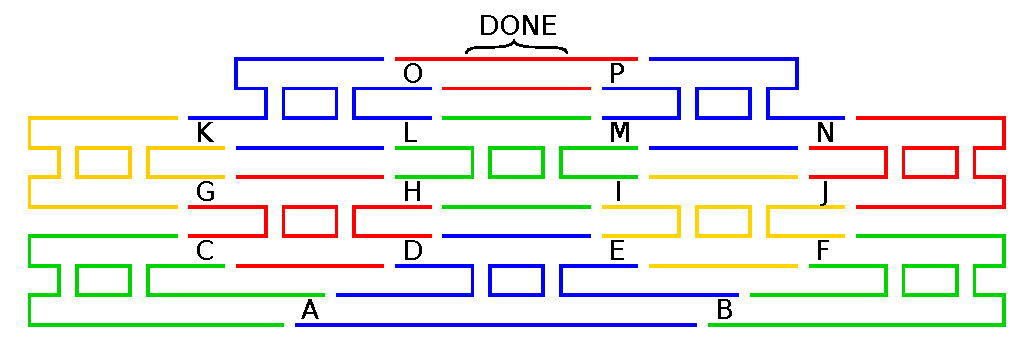
\includegraphics[width=\textwidth]{./figures/tile_model/DNA_assembly.pdf} % 175mm
		\caption{Scheme of self-assembly}
		\label{fig:DNA_assembly}
	\end{subfigure}
	\begin{subfigure}[b]{0.190\textwidth}
		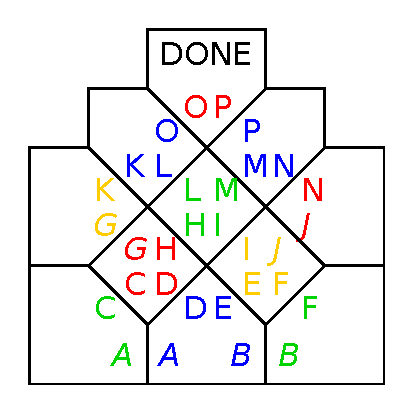
\includegraphics[width=\textwidth]{./figures/tile_model/abstract_model.pdf} % 70mm
		\caption{Abstract model}
		\label{fig:abstract_model}
	\end{subfigure}
	\caption{Evolution of $\myatam$ model from DAE units to tiles. Here italic glues {\sf A}, {\sf B}, {\sf G} and {\sf J} are of strength $2$.} %!% okomentovat že se nic neposere těma lepidlama = 2 na krajích
	\label{fig:evolution}
\end{center}
\end{figure}

\subsection{Feasibility of the class $\BPP$}
	
	As it is often conjectured that the class $\P$ is the class of somehow practically feasible problems, here we introduce similar conjecture for feasible DNA algorithms. The corresponding debate can be found in \cite{book_comp}. %!% najít a citovat delší filozofickou rozpravu
	
	\begin{conj}   %!% conjecture nebo lépe?
		Feasible DNA algorithms comply $Bs(n)\in O(1)$; $Bnd(n),\,Ti(n),\,Gl(n)\in \P$.   %!% možná postačí pro poly algoritmus mín jak \P tile a glue !!! ale spíš ne
	\end{conj}
	
	\begin{thm}   %!% tohle je potřeba někde najít a citovat
		Probabilistic Turing machine can be simulated by probabilistic cellular automaton.
	\end{thm}
	
	\begin{proof}
		Can be found in \ldots
	\end{proof}
	
	\begin{thm}   %!% nějak pojmenovat model, deterministic version by Winfree
		$\myatam$ can simulate probabilistic cellular automaton.
	\end{thm}
	
	\begin{proof}
		Blabla. % poměrem částeček umim nastavit pravděpodobnosti, zbytek důkazu Winfree
	\end{proof}
	
	\begin{cor}
		$\BPP$ is decidable by $\myatam$.
	\end{cor}
	
	%!% nák rozumně vysvětlit že \NP se dá na PTM docela dobře spočítat
	% The model can practically handle also $\NP$ languages (not theoretically, of course) because 